\section{Motivating Prices}

Let \(X_i = X_i(L_i)\) be the set of possible production vectors of person \(i\)
under labour constraint \(L_i\).
\\
\begin{wrapfigure}{r}{0.4\textwidth}
	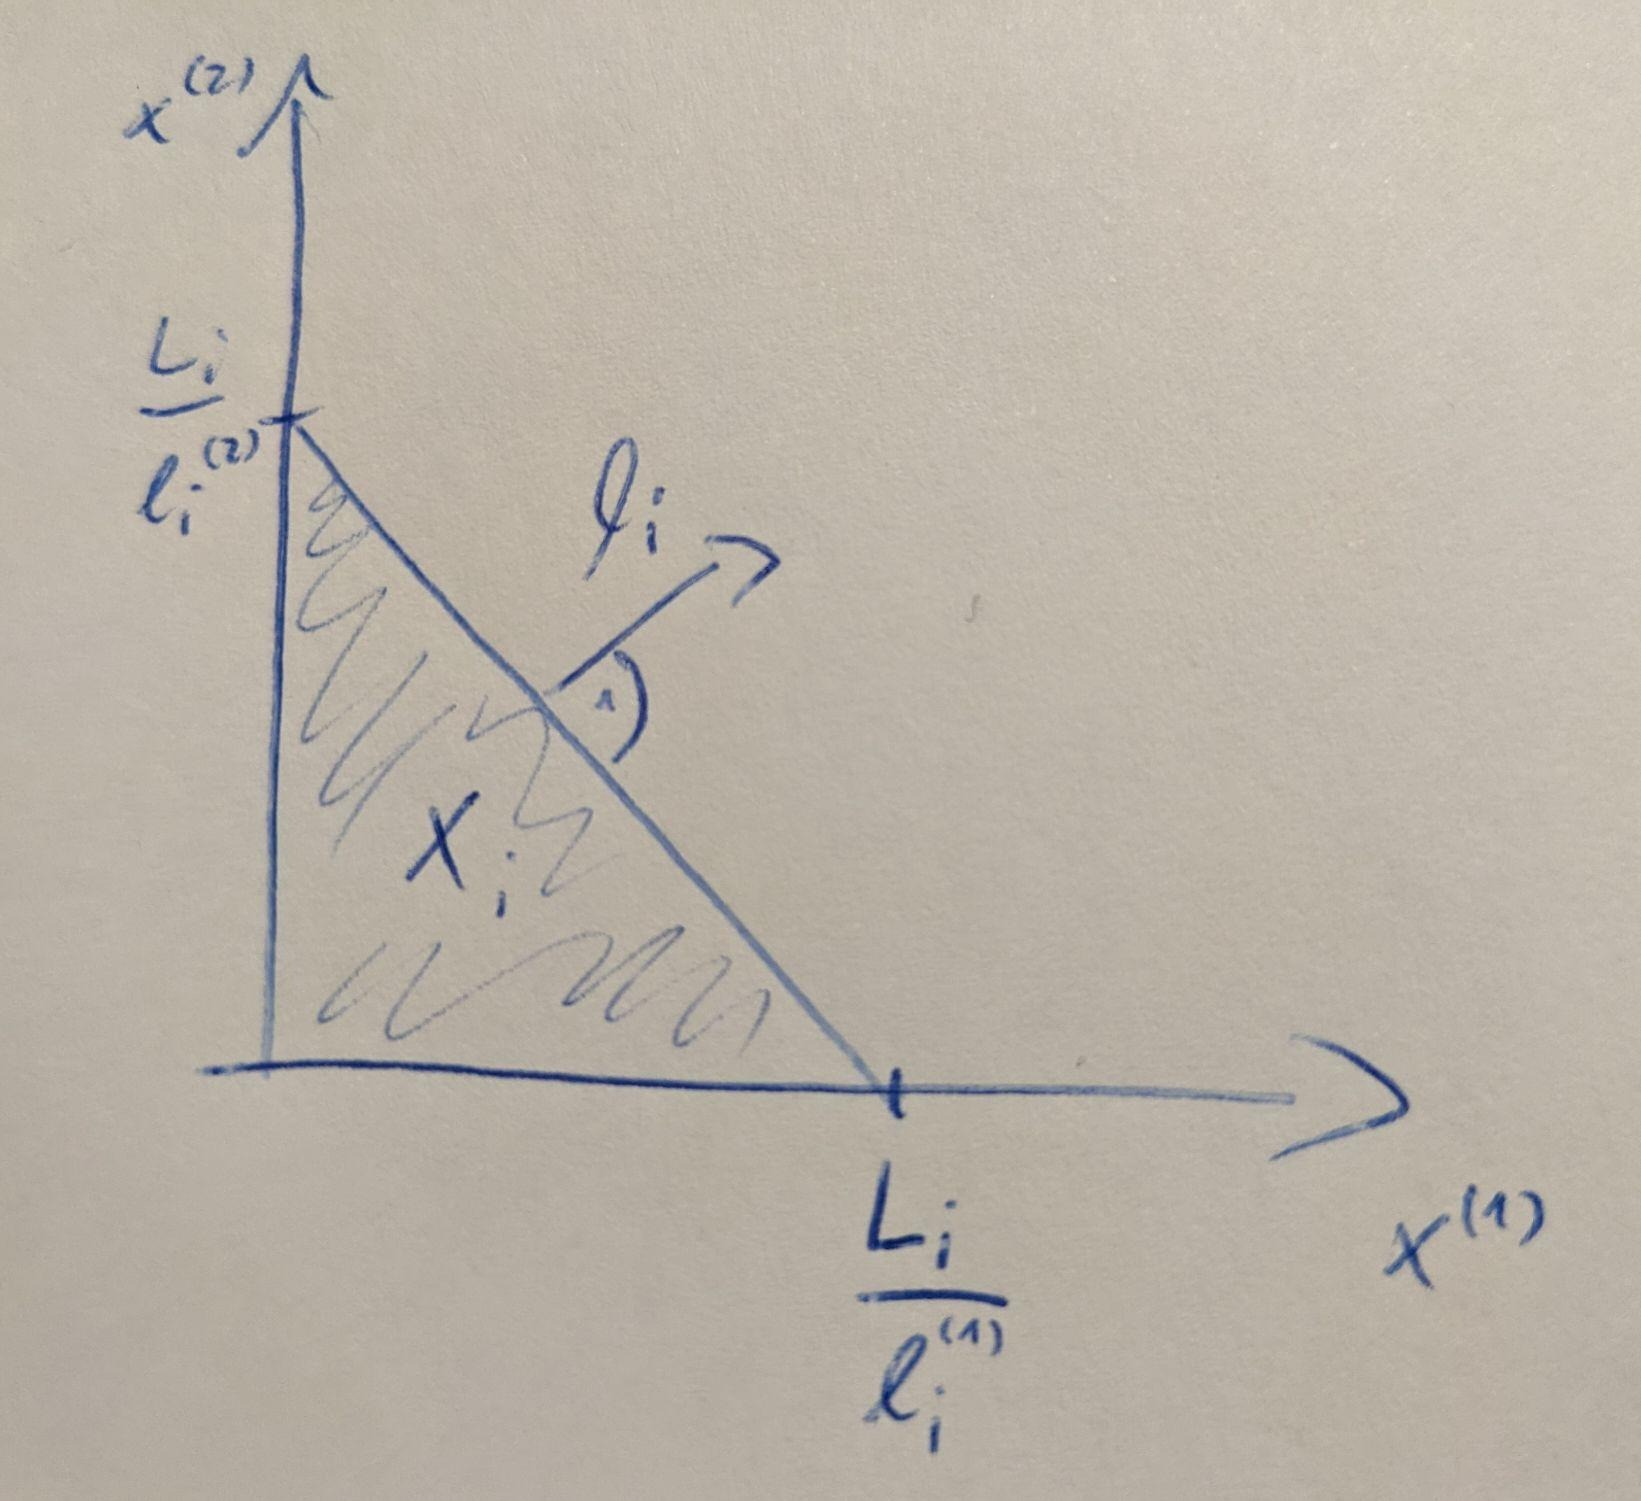
\includegraphics[width=0.4\textwidth]{images/pure-variable-cost.jpeg}
	\caption{Pure Variable Cost \(X_i\)}
\end{wrapfigure}
\begin{example}[Pure Variable Costs]
	One important special case is
	\[
		X_i = \{ x \in \real_{\ge 0}^\dims: \langle x, l_i \rangle \le L_i \}.
	\]
	Here \(l_i^{(j)}\ge0\) is the labour time required by person \(i\) to produce one
	unit of good \(j\). Therefore the total time spent to produce quantity
	\(x^{(j)}\) of good \(j\) is \(x^{(j)}l_i^{(j)}\). Summing over all goods
	results in the total time requirement
	\[
		L_i(x) = \sum_{j=1}^\dims x^{(j)}l_i^{(j)} = \langle x, l_i\rangle,
	\]
	which obviously needs to be smaller than our time constraint \(L_i\).

	One could easily model exhaustion with \(L_i(x) = g(\langle x, l_i\rangle)\)
	for some strictly monotonously increasing function \(g\). You could also
	view \(L_i(x)\) more generally as the discomfort of labour instead of merely
	the time required, to generalize to tasks which take longer but are more
	enjoyable and vice versa.
\end{example}

\begin{example}[Hermit Economy with Pure Variable Costs]
	A hermit faces the utility function maximization problem
	\[
		\max_{x} u(\overbrace{1-L_i(x)}^{\text{free time}}, x).
	\]
	Denoting the partial derivative with regard to free time as \(u_f\) and the
	gradient vector with regard to \(x\) as \(u_x\), the first
	order condition for maximization requires
	\[
		0\overset!=\frac{du}{dx}
		= u_x - \nabla L_i(x) u_f
		= u_f \Bigl[
			\underbrace{\frac{u_x}{u_f}}_{\mathclap{\text{willingness to work (wtw)}}}
		- \overbrace{\nabla L_i(x)}^{\mathclap{\text{natural prices}}}
		\Bigr],
	\]
	where we can assume the marginal utility of more free time \(u_f\) to be
	positive. The natural prices are simply {\color{lightgray} a multiple of}
	\(l_i\)
	\[
		\nabla L_i(x) = {\color{lightgray} g'(\langle x, l_i\rangle) }l_i.
	\]
	In other words: the price of good \(j\), is the {\color{lightgray} marginal}
	time required to produce \(j\). And without exhaustion this is simply
	\(l^{(j)}_i\). If the willingness to work for good \(j\) is smaller than
	its price, then our gradient is negative in this direction. Meaning that
	a reduction of \(x^{(j)}\) would increase our utility. If \(\text{wtw}^{(j)}\) is
	greater than the price of \(j\), an increase of \(x^{(j)}\) increases utility.
\end{example}

Hermits are great and all, but that is not what we are interested in. How could
multiple people share the goods they produced? To satisfy the ``Pluralism in
Economics'' crowd, let us avoid the term ownership for now. We simply observe
that some people will produce things and not necessarily the same people will
use (consume) the products. You can turn a product you can use \(m\) times
(before it breaks down) without loss of generality into a consumable, by
considering these \(m\) uses to be individual products. So a person does not
``have'' a chair, but rather the \(i\)-th usage of said chair. With this trick
in mind, all products are consumable.

No matter how you organize a society, from an individual perspective, there
are going to be goods the individual \(i\) produces \(S_i\in\real^\dims\) and
goods the individual consumes \(D_i\in\real^\dims\). And fundamentally a
society can not consume more than is produced (and probably does not want to
produce more than necessary), so we need
\[
	S = \sum_{i=1}^n S_i = \sum_{i=1}^n D_i = D.
\]
The big question is: how can we ensure this? We also want everyone to
voluntarily participate in society. And people are going to stop doing so, if
they feel ripped off as they contribute much more than they get back.
Unfortunately it is difficult to compare the size of two vectors \(S_i\) and
\(D_i\) of uncomparable products. Of course we could enforce \(S_i=D_i\), but
then we are back to hermits, since everyone is using only what they produce.

To make the products comparable again, we could measure them by the time it took
to produce them. But the time needed to produce good \(j\), \(l_i^{(j)}\), might
be different for every person \(i\). Additionally this time is private
information of person \(i\). Especially if we generalize it to be a discomfort
measure instead of strictly time.


\begin{example}[Definitely not Capitalism]
	\label{ex: Definitely not Capitalism}
	Let us try to build a communist utopia, without money and ownership.  For
	this assume that the person which produces good \(j\) jots down their
	subjective cost of production \(l_i^{(j)}\) and tags the product with it and
	puts it into a communal holding space. Additionally they add the cost to
	their ``work-time'' tally.  Whenever someone wants to consume the product,
	they add the cost to their ``consumption-time'' tally, and take the product
	from communal holding space.  Everyone makes sure that their ``work-time''
	tally is comparable to their ``consumption-time''.

	We can simplify the two tallies into one, because we only want to make
	sure that the difference is approximately zero. So we might as well add
	``work-time'' and subtract ``consumption-time'' from the get go. We also do not
	need to know how the current tally came to be, so we can only keep track of
	the total. This total is going to fluctuate around zero. When it is positive,
	you have worked more for society than you have consumed. And vice versa when it
	is negative.

	Now consider the life of a single product. When it is consumed, the cost was
	added to the tally of the producer and subtracted from the consumer. If you
	had chips to represent the tally, then they would have been simply passed from
	the consumer to the producer. Oh, wait! That's money! People are trading goods
	for money!

	Although right now, tallies can be negative and we do not have negative
	chips/money. This is a problem if you start out with everyone at zero. Because
	nobody can go below that. Or can they? If Ben signs a piece of paper saying
	he owes \(x\) amount of work-time, then he can pass that for a product that
	costs \(x\). The person receiving this note could then pass this note on to
	pay for something too. And if everyone trusts Ben, this is going to go
	swimmingly. So in principle anyone can create money. Money is just the debt of
	someone. The difficulty is creating debt which is widely accepted.

	The balance on a bill splitting app is money (in your friends circle), a coupon
	is money (scammers like to be paid in it), etc. But the money which is most
	widely accepted, is the money issued by a trusted government. Because money is
	debt, so the question whether you accept is, is whether you trust the debtor.
\end{example}
\begin{remark}
	Example~\ref{ex: Definitely not Capitalism} is supposed to show how difficult
	it is to come up with a system which balances production and consumption,
	which is not mathematically equivalent to a market economy. And while the
	initially proposed tally system might be mathematically equivalent, it is
	much less robust and efficient in reality. Because you need to \emph{trust}
	people to update their tallies accurately, \emph{trust} that they make sure
	they don't go too far into the negative, and you need to travel to a
	communal holding space instead of conducting exchanges decentrally.
\end{remark}





\begin{figure}
	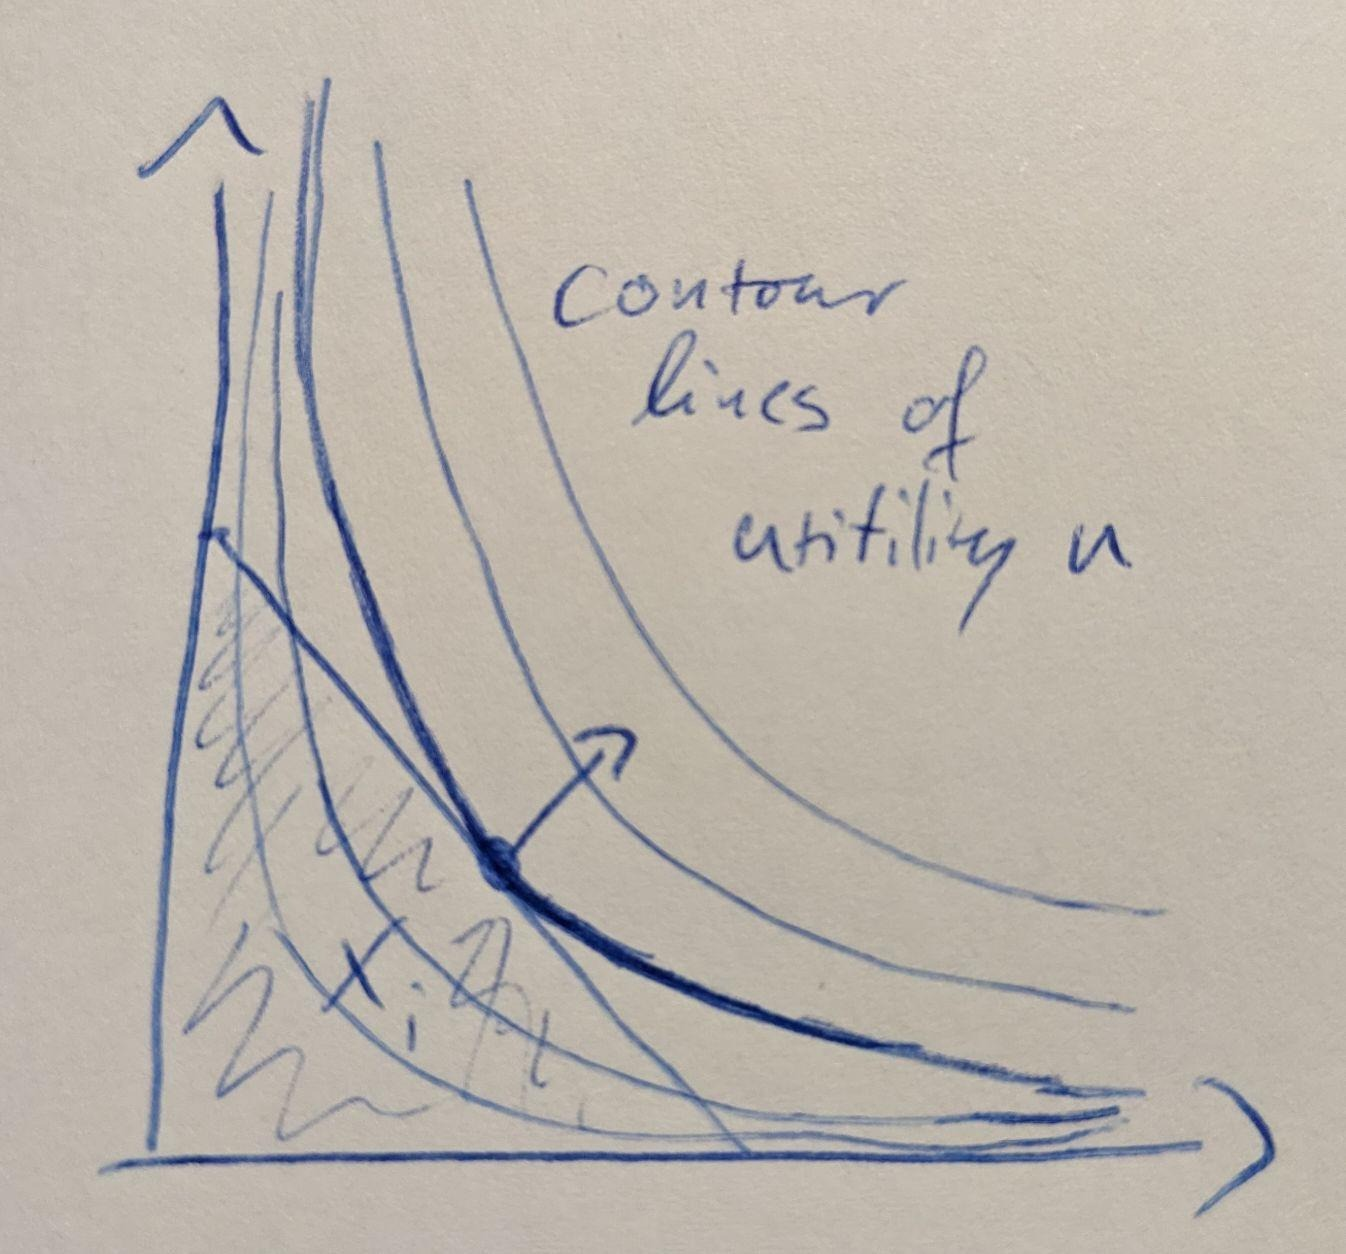
\includegraphics[width=0.4\textwidth]{images/hermit-decision-pure-variable.jpeg}
	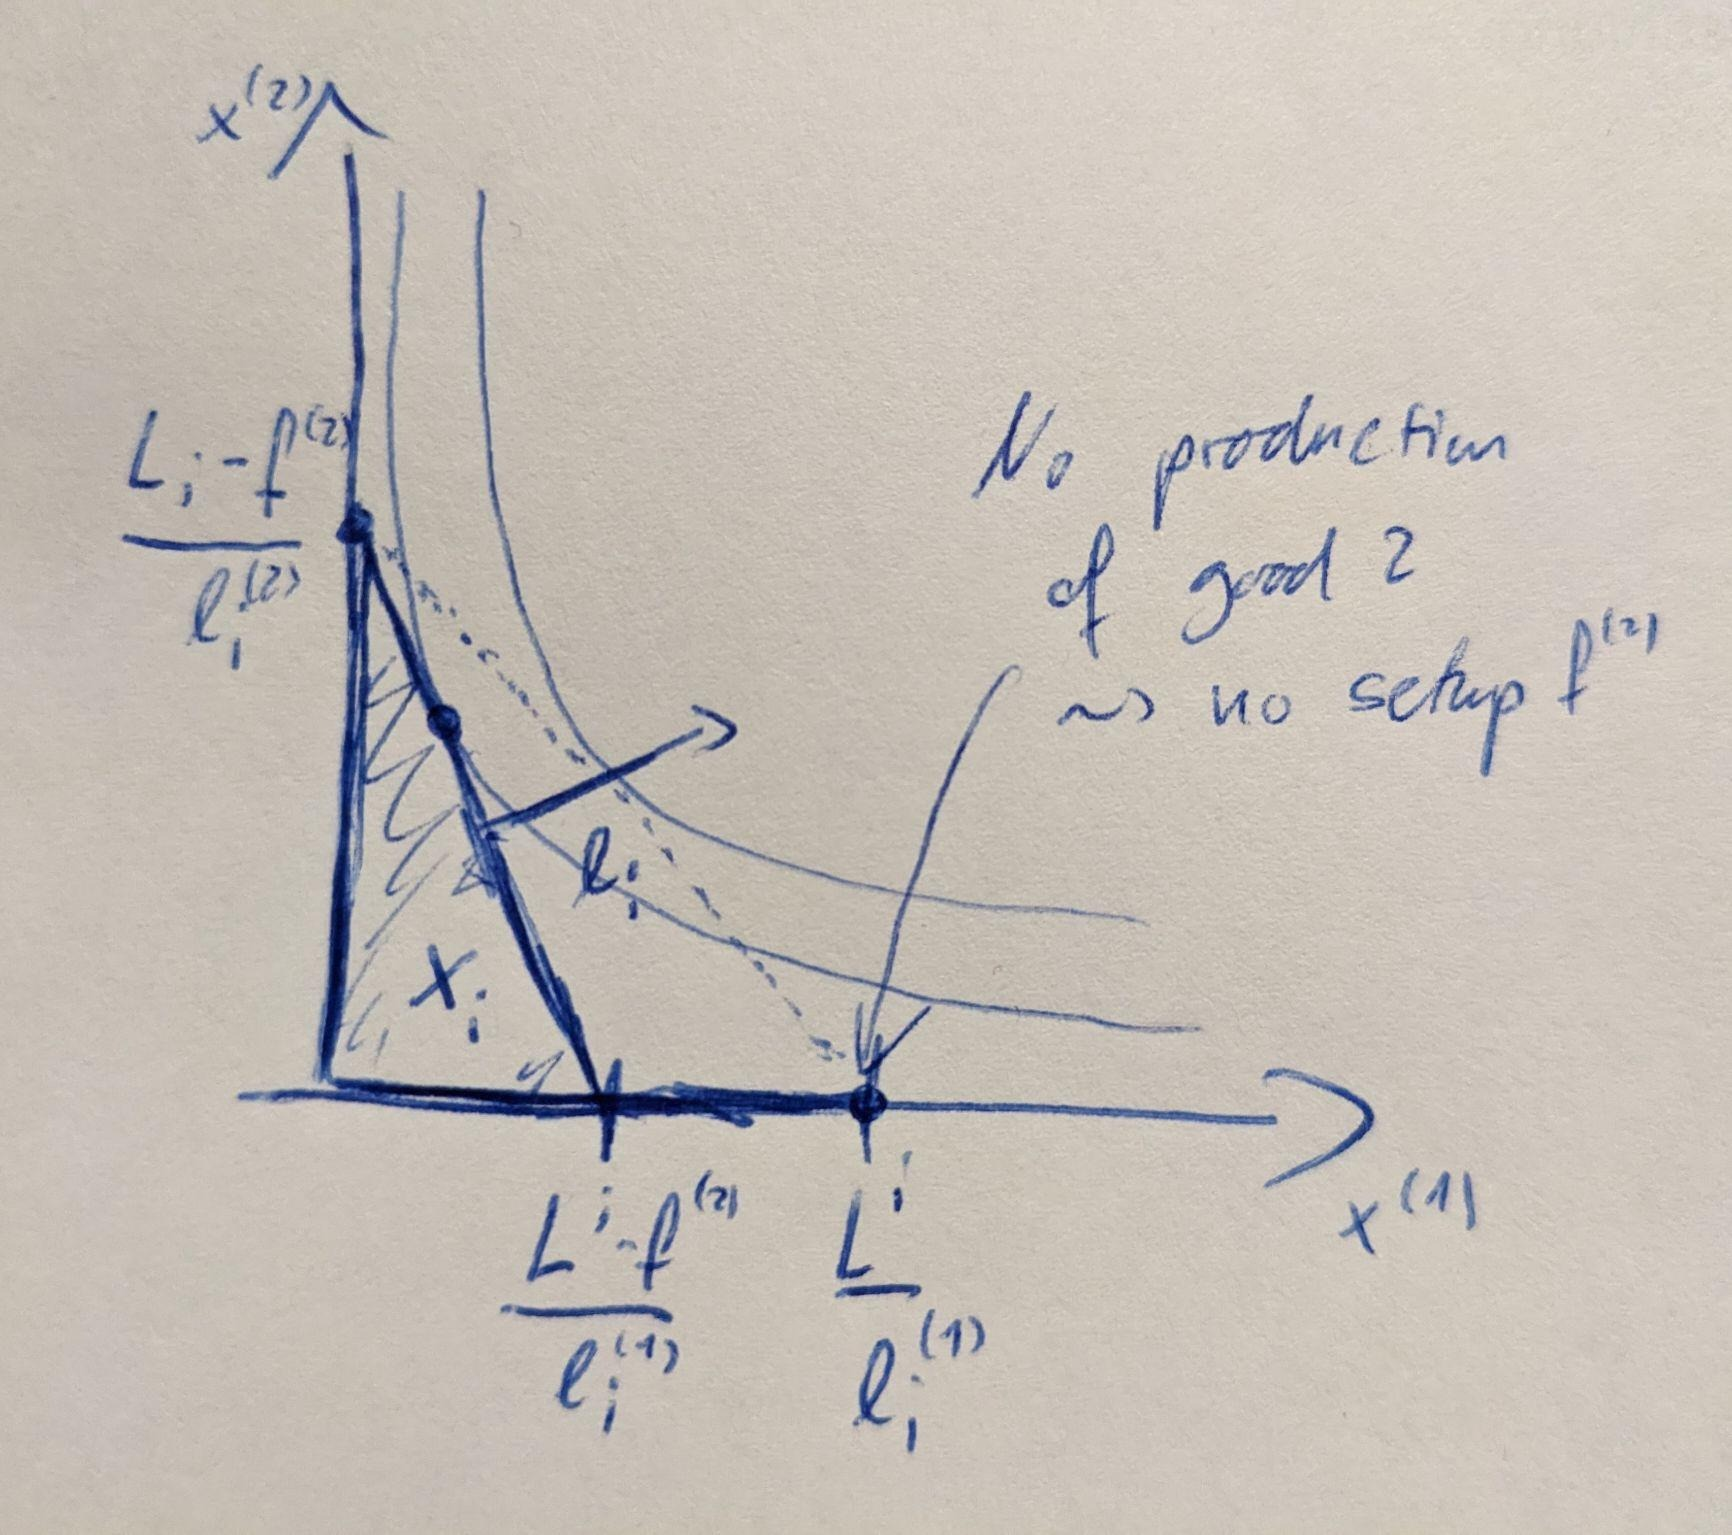
\includegraphics[width=0.58\textwidth]{images/hermit-decision-setup-cost.jpeg}
	\caption{Hermit Decision in simple pure variable cost case on the left.
	fixed set-up time \(f^{(2)}\) for the production of good \(2\) to the right.
	This allows for more production of good \(1\) if \(x^{(2)}=0\). The dotted
	line represents the production frontier in the ``cloned hermit economy''.}
\end{figure}
\begin{example}[Cloned Hermit Economy]
	If we clone our hermit in the previous example \(n\) times, the clones could
	start trading. Although they have very little reason to do so for now.
	Nevertheless let us first consider what exchange rates are possible before
	we modify \(X_i\) to give them a reason to do so.
\end{example}
